\documentclass[border=2mm]{standalone}
\usepackage{pgfplots}
\pgfplotsset{compat=1.18}
\usetikzlibrary{arrows.meta, calc, positioning, decorations.pathreplacing, calligraphy}

\usepackage{xcolor}
\definecolor{den-1}{HTML}{111111}   % Đen #111111
\definecolor{den-2}{HTML}{222222}   % Đen #222222
\definecolor{den-3}{HTML}{333333}   % Đen #333333
\definecolor{den-4}{HTML}{444444}   % Đen #444444
\definecolor{den-5}{HTML}{555555}   % Đen #555555
\definecolor{den-6}{HTML}{666666}   % Đen #666666

\definecolor{do-1}{HTML}{440000}   % Đỏ #440000 trầm hơn, hợp với đen #111111
\definecolor{do-2}{HTML}{660000}   % Đỏ #660000 sẫm, hợp với đen #222222
\definecolor{do-3}{HTML}{880000}   % Đỏ #880000 đậm vừa, hợp với đen #333333
\definecolor{do-4}{HTML}{AA0000}   % Đỏ #AA0000 tươi vừa, hợp với đen #444444
\definecolor{do-5}{HTML}{CC0000}   % Đỏ #CC0000 tươi hơn, hợp với đen #555555
\definecolor{do-6}{HTML}{EE0000}   % Đỏ #EE0000 sáng hơn, hợp với đen #666666

% Thiết lập vị trí đặt nhãn gốc tọa độ
\tikzset{
  >=Stealth,
  originlabel/.style={
    font=\small\sf,
    anchor=north east, % Vị trí tương đối so với gốc
    yshift=-0.1ex,     % Điều chỉnh vị trí dọc một chút
    xshift=-0.1ex      % Điều chỉnh vị trí ngang một chút
  }
}

\begin{document}
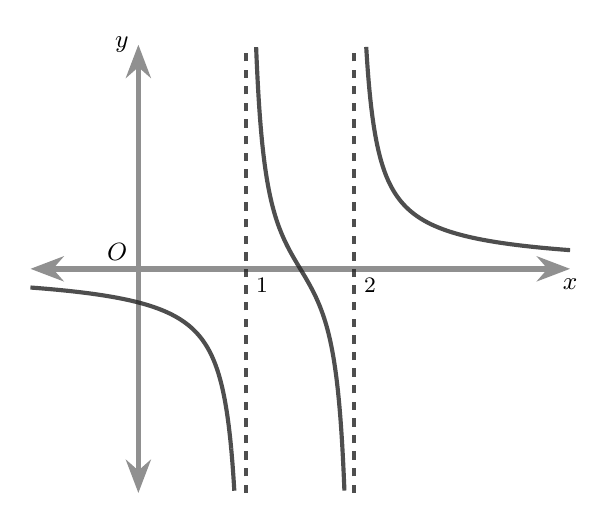
\begin{tikzpicture}
  \begin{axis}[
    font=\small\sf,
    axis lines = middle,
    axis line style={<->, line width=2pt, color=den-2!50},
    xlabel=$x$, ylabel=$y$,    
    xlabel style={below, font=\small\sf},
    ylabel style={left, font=\small\sf},
    xmin=-1, xmax=4,
    ymin=-2, ymax=2,
    xtick=\empty, ytick=\empty,
    tick label style={font=\footnotesize\sf, /pgf/number format/use comma=false, /pgf/number format/1000 sep={}},
    clip=false,
    domain=-1:4,
    samples=400,
    restrict y to domain=-2:2,
  ]

  \node[originlabel] at (axis cs:0,0) [above left] {$O$};
  \node at (axis cs:1,0) [anchor=north west] {\footnotesize$1$};
  \node at (axis cs:2,0) [anchor=north west] {\footnotesize$2$};
  
  \addplot[domain=-1:0.86, color=den-2, line width=1.5pt, opacity=.8] {(2*x - 3)/(5*x^2 -15*x +10)};
  \addplot[domain=0.86:2.14, color=den-2, line width=1.5pt, opacity=.8] {(2*x - 3)/(5*x^2 -15*x +10)};
  \addplot[domain=2.14:4, color=den-2, line width=1.5pt, opacity=.8] {(2*x - 3)/(5*x^2 -15*x +10)};

  % Tiệm cận đứng
  \addplot[dashed, color=den-2, line width=1.5pt, opacity=.8] coordinates {(1,-2) (1,2)};
  \addplot[dashed, color=den-2, line width=1.5pt, opacity=.8] coordinates {(2,-2) (2,2)};

  \end{axis}
\end{tikzpicture}
\end{document}
